\section{Introdução e Justificativas}\label{Intro}


%=============================================================================
% 							INTRODUÇÃO
%=============================================================================

%GFC E QUESTIONAMENTO DO INVESTIMENTO COMO CAUSA CAUSANS

%INTRODUÇÃO MAIS LONGA: EUA E CRISE

Nos Estados Unidos (EUA), o início dos anos 2000 é demarcado por momentos bastante distintos. Logo em 2001, a economia é atingida pela crise das bolhas-ponto-com com a possibilidade de uma recessão. No entanto, a recuperação foi rápida e seguida de um ciclo de crescimento que se estendeu de 2002 a 2007 \cite{cagnin_o_2007}. Apesar desta dinâmica sugerir uma atipicidade, segue um padrão bem definido para o caso norte-americano, qual seja, o ciclo econômico é liderado pelo investimento residencial \cites{green_follow_1997}{leamer_housing_2007}{fiebiger_trend_2017}\footnote{
	Ao avaliar o caso norte-americano, \textcite{green_follow_1997} conclui que o investimento residencial antecipa o ciclo econômico mas que isso não implica no estabelecimento de uma relação causal. 
}. Apesar da economia americana seguir crescendo até 2007, o investimento residencial iniciou a reversão já em 2005. Ao longo deste período, os demais componentes da demanda agregada contribuíram para o adiamento da crise, mas não foram suficientes para impedir o colapso do investimento residencial ocorrido em 2008. 

A crise \textit{subprime} de 2008, antes uma crise focalizada no mercado imobiliário americano, ampliou-se em uma crise financeira que tomou dimensões globais. Além das mudanças sócio-econômicas, a crise teve implicações para a teoria econômica. Se, por um lado, abalou a macroeconomia ortodoxa ao ponto da política fiscal estar sendo repensada \cite{blanchard_rethinking_2017}, por outro, redirecionou algumas pautas na heterodoxia. Distribuição e desigualdade, temas tão caros a esta última tradição, ganharam novo fôlego\footnote{Cabe pontuar que até o \textit{mainstream} passou a se dedicar ao assunto com destaque ao trabalho de \textcite{piketty_o_2014}.} \cites{carvalho_personal_2016}{ederer_will_2019} enquanto parte da literatura passou a destacar o consumo como um dos possíveis motores de crescimento\footnote{Para uma resenha da literatura recente sobre o consumo, ver \textcite{brochier_macroeconomics_2017}}. Paralelamente, verificou-se um crescente interesse nas implicações macroeconômicas do investimento residencial\footnote{E isso é verificado até na literatura ortodoxa. Inspecionando modelos DSGE que incluem investimento residencial, \textcite{iacoviello_housing_2010} conclui que um melhor entendimento dos impactos deste gasto se faz necessária para a compreensão das flutuações macroeconômicas.} \cites{teixeira_crescimento_2015}{fiebiger_semi-autonomous_2018} e é justamente nesta agenda de pesquisa que essa investigação se insere. 

Neste ponto, cabe mencionar o ineditismo de \textcite{green_follow_1997} e \textcite{leamer_housing_2007} --- revisitado em \textcite{leamer_housing_2015} e por \textcite{fiebiger_semi-autonomous_2018} --- ao lançar luz sobre a importância do investimento residencial na determinação dos ciclos econômicos nos EUA em todo o pós-guerra.
Antes mesmo da crise no mercado imobiliário,
\textcite{leamer_housing_2007} destaca a capacidade preditiva e relação causal  do investimento residencial com o PIB. Sucintamente, afirma que a construção de novos imóveis permite, via aumento das linhas de crédito, um maior consumo de bens duráveis e, portanto, o ciclo econômico americano pode ser configurado como um \textit{consumer cycle} e não como um \textit{business cycle}.

Da revisão de literatura, verificou-se que a fronteira tem avançado em três frentes. Uma delas trata da importância do investimento residencial para o ciclo econômico por meio de modelos macroeconométricos.
Outra frente  diz respeito a importância das instituições para a compreensão dos impactos deste gasto para a dinâmica macroeconômica enfatizando as relações entre mercado imobiliário, de crédito e endividamento das famílias. 
Por fim, uma parcela menor direciona esforços para conectar o investimento das famílias nas teorias de crescimento. Esta pesquisa irá avançar nestas direções e suprir algumas das lacunas que serão destacadas adiante.

Apesar da relevância do investimento residencial para a dinâmica macroeconômica não se restringir aos EUA, parte expressiva desta literatura tem centrado esforços neste caso em específico. A razão disso é que os imóveis são  uma das formas de riqueza mais comuns entre as famílias norte-americanas e serviam --- principalmente nos anos 2000 --- de colateral para tomada de crédito \cite{teixeira_uma_2011}. A forma de ``realizar'' o ganho de capital com a bolha imobiliária que ocorreu no período, sem precisar liquidá-los, era justamente ampliando o endividamento à medida que este colateral aumentava de valor \cite{teixeira_crescimento_2015}. Nesses termos, evidencia-se os impactos da bolha de ativos sobre a demanda agregada. 


Uma análise que complementa os efeitos do investimento residencial sobre a dinâmica financeira é a da ``hipotecarização''. 
Desenvolvida por \textcite{jorda_great_2014}, esta hipótese destaca a crescente participação das hipotecas nos balanços patrimoniais dos bancos de ao menos 17 países da OCDE\footnote{\textcite{jorda_great_2014} também destacam que o crédito hipotecário era concedido fora do sistema bancário até os 1900 e isso dificulta a estimação dos dados.}\footnote{Paralelamente, os autores pontuam que os empréstimos às famílias têm aumentado a uma velocidade superior ao valor de seus ativos e, portanto, verifica-se uma maior alavancagem --- logo, maior fragilidade financeira das famílias --- apesar do aumento do preço dos imóveis.} (ver figura \ref{GraficoJorda}).
Apesar de esclarecer as relações entre investimento residencial (lado real) e balanço patrimonial dos bancos (lado financeiro), tal contribuição não tem sido investigada sob um ponto de vista pós-keynesiano em que as relações financeiras entre os diferentes agentes institucionais desempenham um papel central. Para ilustrar a compatibilidade desta hipótese a esta tradição, tal contribuição permite destacar os efeitos do investimento residencial sobre a dinâmica financeira: 

\begin{quote}
	\textit{To a large extent the core business model of banks in advanced economies today resembles that of real estate funds: banks are borrowing (short) from the public and capital markets to invest (long) into assets linked to real estate.} [...] \textit{looking more deeply at the composition of bank credit, it becomes clear that the rapid growth of \textbf{mortgage lending} to households has been the \textbf{driving force} behind this remarkable change in the composition of banks’ balance sheets} \cite[p.~2, grifos adicionados]{jorda_great_2014}
\end{quote}
Além disso, a partir da base de dados desenvolvida --- e em constante atualização --- pela equipe de Jordà, uma investigação mais aprofundada desta hipótese abre uma agenda de pesquisa sobre a importância do investimento residencial para a dinâmica macroeconômica que vai além dos EUA e se estende para alguns países da OCDE. Nesses termos, a presente pesquisa se justifica pela necessidade de uma maior compreensão 
%do papel das hipotecas no sistema bancário bem como 
da relação entre investimento residencial e dinâmica macroeconômica dados os impactos reais e financeiros que este componente da demanda agregada tem sobre o ciclo econômico. 

\begin{figure}
	\centering
	\caption{Participação do empréstimo imobiliário no total do balanço patrimonial dos bancos (1870-2016)}
	\label{GraficoJorda}
	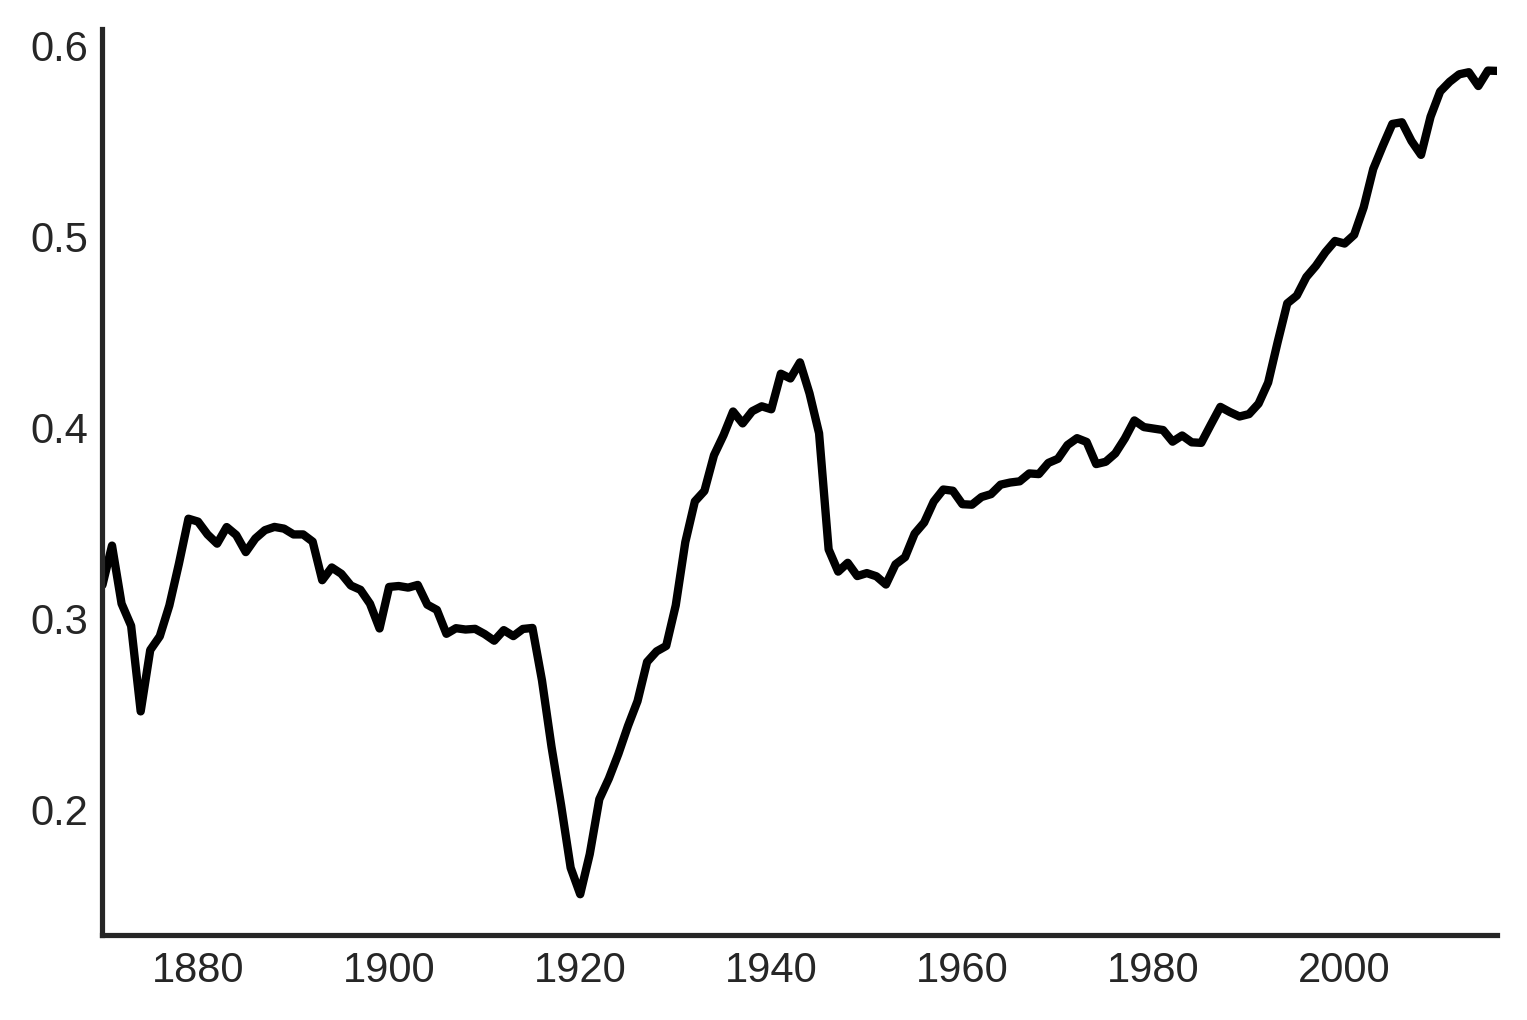
\includegraphics[width=.65\textwidth]{Jorda_Mean.png}
	\caption*{\textbf{Fonte:} \textcite[p.~10]{jorda_great_2014}}
\end{figure}


%Desse modo, uma das consequências no pensamento macroeconômico heterodoxo é o debate a respeito do papel do investimento das firmas enquanto ``causa das causas''. 

No que diz respeito ao ciclo econômico, parte da literatura econométrica também tem lançado luz sobre a importância do investimento residencial e tal relevância não se restringe à crise \textit{subprime} nem aos EUA. \textcite{alvarez_does_2010}, por exemplo, concluem que tal tipo de investimento antecede o ciclo econômico para o caso espanhol e resultados semelhantes podem ser encontrados para França, Espanha  e Itália enquanto o caso alemão apresenta uma dinâmica distinta \cites{ferrara_cyclical_2010}{ferrara_common_2010}. 
Outros estudos empíricos, por sua vez, têm enfatizado o efeito riqueza --- via valorização dos imóveis --- sobre o consumo e indicam tais canais de transmissão são mais incidentes, em ordem, sobre Estados Unidos e Grã Bretanha e mais brandos no caso francês e alemão \cites{sastre_assessment_2010}{chauvin_wealth_2010}{bassanetti_effects_2010}{arrondel_housing_2010}.

%INSTITUIÇÕES

A pluralidade de resultados reportada acima sugere que a especificidade institucional de cada país desempenha um papel central nas implicações macroeconômicas do investimento residencial e, portanto, carece de uma investigação mais detalhada.
A título de exemplo, \textcite{wijburg_alternative_2017} destacam que a especificidade instucional do mercado imobiliário alemão\footnote{Os autores também apontam que os preços dos imóveis na Alemanha estagnaram enquanto o resto do mundo presenciou um aumento. No entanto, observa-se um movimento recente de aumento nos preços no país, indicando uma maior relevância do tema em um futuro próximo.} o configura como um contra ponto ao norte-americano:

\begin{quote}
On the one hand, the German housing
market was one of the few markets in Western Europe that was not severely affected by the
global housing boom of the early 2000s. On the other hand, recent developments suggest
that the role of finance in the German housing system is \textbf{changing}, but not in the same way as
in other countries. \cite[p.~969, grifos adicionados]{wijburg_alternative_2017}
\end{quote}
Também seguindo uma análise das instituições, \textcite{van_gunten_varieties_2018} argumentam que as mudanças institucionais ocorridas desde a década de 90 foram responsáveis pela maior intensificação financeira das famílias\footnote{Isto é, maior endividamento das famílias e não um aumento no número de famílias endividadas.} em Portugal e Espanha se comparado com França e Alemanha. Sendo assim, para uma melhor compreensão das inter-relações entre o mercado imobiliário e o de crédito, se faz necessário destacar a importância das instituições\footnote{
	Ao longo desta pesquisa, adota-se a definição de instituições como em 	\textcite[p.~85]{dequech_economic_2013}: ``\textit{Institutions are broadly understood here as socially shared systems of rules of behavior or of thought that have some recurrence}'' e, mais especificamente, serão avaliadas as instituições formais.}.  


Pontuada a importância do investimento residencial e a relevância das instituições para compreendê-lo, cabe inspecionar a forma com que a heterodoxia tratou do tema. Parte significativa desta literatura  --- emergente no pós-crise --- centra esforços na conexão deste tipo de gasto com processos mais gerais como a financeirização \cites{aalbers_financialization_2008}{bibow_financialization_2010} enquanto uma fração minoritária o relaciona com as variabilidades de capitalismo e as relações com o \textit{welfare state} \cite{schwartz_politics_2009}. 
No entanto, a partir da revisão bibliográfica, verificou-se que uma fração pequena da literatura heterodoxa\footnote{
	A título de menção, vale destacar também o trabalho de \textcite{zezza_u.s._2008} em que são investigados os efeitos distributivos sobre o crescimento para a economia norte-americana a partir da metodologia \textit{Stock-Flow Consistent}.}
aborda as relações entre crescimento e investimento residencial\footnote{A título de nota, destaca-se que debate ortodoxo sobre desenvolvimento e investimento residencial centrado na década de 60-70 (ver \textcite{arku_housing_2006}) se restringiu em categorizá-lo como um gasto absorvedor de recursos produtivos e indicava  a possibilidade de um sobreinvestimento residencial \cites{solow_importance_1995}{mills_has_1987}. }. 
Uma forma de incluir esse gasto nos modelos de crescimento heterodoxos é a de \textcite{teixeira_crescimento_2015} --- retomada em \textcite{da_silveira_investimento_2019} --- em que é utilizado o modelo do tipo supermultiplicador sraffiano (SSM em inglês) por estabelecer um papel fundamental aos gastos autônomos que não criam capacidade no crescimento econômico e na acumulação de capital.



Na contribuição original de \textcite{serrano_sraffian_1995} e nas apresentações mais recentes \cite{freitas_growth_2015}, o modelo é apresentado de modo bastante parcimonioso para evidenciá-lo como um fechamento alternativo, dentro da tradição da teoria do crescimento liderada pela demanda \cite{serrano_sraffian_2017}. 
Sucintamente, o SSM descreve um padrão de crescimento liderado pela demanda em que os gastos autônomos não criadores de capacidade produtiva (ditos improdutivos) determinam a taxa de crescimento de longo prazo. 
Nesta família de modelos: 
	(i) o grau de utilização converge ao grau normal (planejado pelas firmas) no longo prazo; 
	(ii) a distribuição renda não influencia o crescimento de longo prazo; 
	(iii) o investimento das \textbf{firmas} segue o princípio de ajuste do estoque de capital e;
	(iv) o ajuste do estoque de capital é feito de forma tênue e gradual. 
	
Uma forma de conectar o investimento residencial com o modelo do supermultiplicador sraffiano é por meio da taxa de juros real dos imóveis desenvolvida por \textcite{teixeira_crescimento_2015}\footnote{Na contribuição de \textcite{teixeira_crescimento_2015}, tal taxa é denominada de Taxa Própria de Juros do Imóveis. Para evitar complicações, optou-se por tratá-la como uma taxa de juros real específica.} para avaliar o caso norte americano. Nesta formulação, a taxa de juros das hipotecas capta o serviço da dívida para os ``investidores'' (neste caso, famílias) enquanto a variação do preço dos imóveis permite incorporar mudança no patrimonio líquido\footnote{Em linhas gerais, esta taxa real de juros aufere de modo satisfatório o custo real em imóveis de se comprar imóveis \cite[p.~53]{teixeira_crescimento_2015}. Tal proposta, portanto, lança luz sobre a influência da inflação imobiliária na construção de novos imóveis e, de acordo com o SSM, na determinação do nível e da taxa de crescimento do produto.}. 
A partir deste tipo específico de taxa de juros real, portanto, é possível introduzir inflação de ativos nos modelos do tipo SSM. No entanto, a referida taxa foi desenvolvida para examinar a bolha de ativos ocorrida nos EUA e, portanto, não foi feita uma investigação a despeito da aplicabilidade para outros países e este é um dos objetivos desta pesquisa.

	
Vale ressaltar que a partir do estabelecimento do SSM, algumas questões são colocadas: quais são esses gastos autônomos e quais seus determinantes? Qual o padrão de financiamento e suas consequências? \textcite{pariboni_household_2016} e \textcite{fagundes_dinamica_2017}, por exemplo, avançaram em detalhar o consumo financiado por crédito.  \textcite{brochier_supermultiplier_2018}, por sua vez, incorporam o SSM em uma estrutura contábil mais completa, o arcabouço de consistência entre fluxos e estoques (SFC, na sigla em inglês), para compreender a dinâmica do consumo a partir da riqueza. Outro modelo que une o SSM a metodologia SFC é o de \textcite{da_silveira_investimento_2019}. Tal contribuição, apesar de analisar a dinâmica de dois tipos distintos de estoques de capital (das firmas e das famílias), carece de uma relação entre o mercado imobiliário e de crédito bem como uma maior ênfase no endividamento das famílias e na inflação de ativos, portanto, tal modelo pode --- e precisa --- ser  aprimorado.


Como será discutido adiante, a ênfase em tratar a abordagem SFC enquanto uma metodologia decorre da flexibilidade de incluir inúmeras teorias e propostas em um arcabouço contábil rígido\footnote{Apenas para ilustrar a pluralidade de temas que tal metodologia já abordou, temos --- mesmo que em sua forma mais originária encontrada em \textcite{godley_macroeconomics_1983} --- as formas de financiamento das firmas \cites{asimakopulos_kalecki_1983}{skott_finance_1988}{messori_financing_1991}; endogeneidade da moeda e importância do sistema bancário \cites{messori_financing_1991}{dow_horizontalism:_1996}{arestis_theoretical_1996}{godley_money_1999}; endividamento, distribuição de renda e, apenas para restringir os temas, financeirização \cites{palley_inside_1996}{wolfson_irving_1996}{palley_money_1997}{palley_financial_2002}{dos_santos_revisiting_2009}{palley_inside_2010}{hein_finance-dominated_2012}.}. 
A mesma variabilidade de temas possíveis de serem abordados pela metodologia SFC se estende para a pluralidade dos ativos passíveis de serem incorporados e ao grau de complexidade financeira de cada modelo. Uma forma de visualizar tal flexibilidade é por meio da figura \ref{Heatmap} em que são mapeados os ativos mais frequentes. No entanto, esta figura também revela que a literatura não dá a devida atenção ao investimento residencial\footnote{Deve ser pontuada a notória exceção de \textcite{zezza_u.s._2008} em que é apresentado um modelo com imóveis em um aparato Kaleckiano enfatizando as implicações distributivas mas não trata de questões envolvendo ganhos de capital ou dos determinantes do investimento residencial.}, sendo o ativo menos estudado. 


Uma vez que a dívida hipotecária é o principal componente do endividamento das famílias, se faz necessária uma melhor compreensão da conexão entre o investimento residencial com as formas de financiamento e estoques financeiros de forma integrada.
Nesses termos, a abordagem SFC se mostra a mais adequada para o tipo de análise pretendido. Portanto, fica evidenciada a lacuna que esta pesquisa procurará preencher.
Sendo assim, um modelo de crescimento do tipo SSM com a metologia SFC (adiante, SSM-SFC) se mostra como uma alternativa para tratar do investimento residencial em que são mapeadas as relações financeiras entre os diferentes agentes institucionais.

\begin{figure}[htb]
	\centering
	\caption{Mapa de calor dos ativos modelados com SFC}
	\label{Heatmap}
	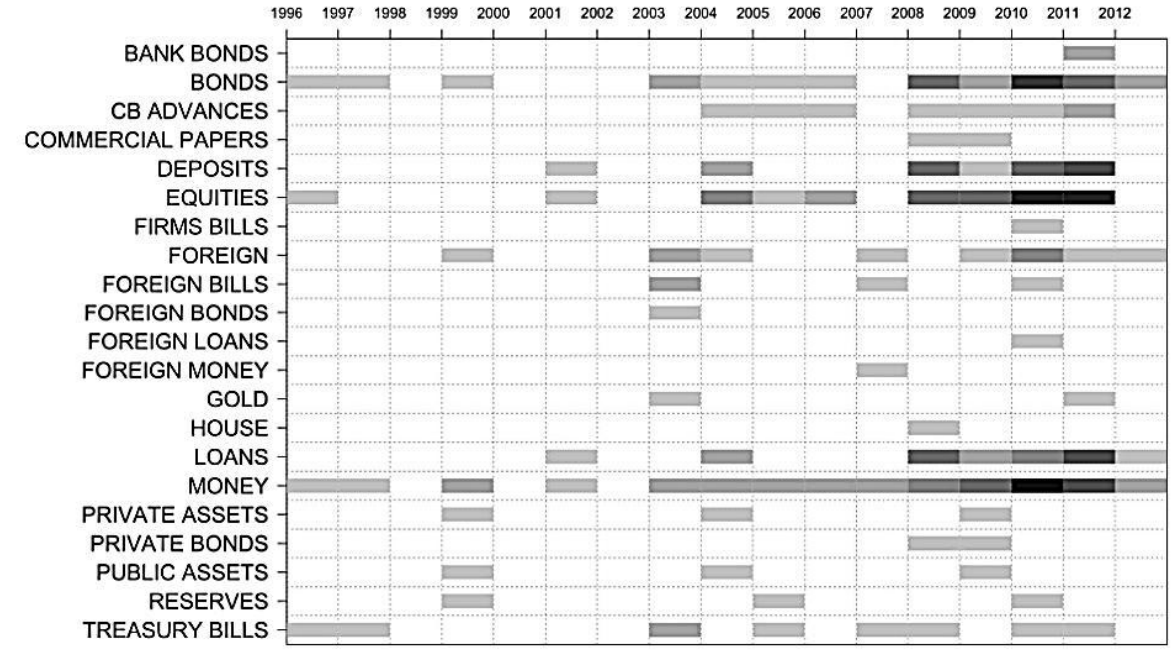
\includegraphics[width = 0.9\textwidth]{../../Escrita_Dissertacao/Da_Silveira_Dissertacao_Atual/Modelo/Caverzassi_Heatmap.png}
	\caption*{\textbf{Fonte:} \textcite[p.~4]{caverzasi_stock-flow_2013}}
\end{figure}




%PERGUNTA
Compreendido este panorama, a presente investigação tem como objetivo estudar as relações entre investimento residencial e dinâmica macroeconômica. Em particular, pretende-se analisar as relações entre mercado imobiliário e de crédito tendo em vista elementos teóricos e institucionais. Dito isso, esta pesquisa busca responder a seguinte pergunta: quais os principais determinantes institucionais que explicam as relações entre investimento residencial e dinâmica macroeconômica? 
Compreendidas tais relações, será desenvolvido um modelo SSM-SFC para dar conta das relações entre lado real e financeiro da economia.
Portanto, esta pesquisa segue o caminho aberto por \textcite{brochier_supermultiplier_2018} ao adicionar um tratamento adequado das relações financeiras no SSM por meio da metodologia SFC estentendo as contribuições de: 
(i) \textcite{jorda_great_2014} ao investigar o processo de ``hipotecarização'' sob um prisma pós-keynesiano; 
%(ii) \textcite{serrano_sraffian_1995} ao incluir o investimento residencial na agenda de pesquisa do supermultiplicador sraffiano; 
(ii) \textcite{teixeira_crescimento_2015} ao avaliar a aplicabilidade da taxa própria de juros dos imóveis para além dos Estados Unidos e;
(iii) \textcite{da_silveira_investimento_2019} ao conectar as relações entre o mercado imobiliário e de crédito diante das especificidades institucionais destacas anteriormente assim como a endogeinização da inflação de imóveis. 